% author: Simon Bachmann

\section{Social Trust Certificates}\label{section:social-trust-certificates}

A decentralized ticketing platform does not restrict any user from creating an event on the distributed ledger. Thus, a mechanism must be developed to mitigate fraudulent events. 

Social trust certificates enable a user to check whether the event is legitimate or not without the need of a third party. By uploading the same public key, that is used for creating the event, to a social profile or the official event website, an event host can proof his ownership of the event as well as the social profile or website. 

Figure \ref{fig:trust-certificate-event-website} illustrates how the event host can use the official event website to increase the authenticity of the event. 

\begin{figure}[H]
    \centering
    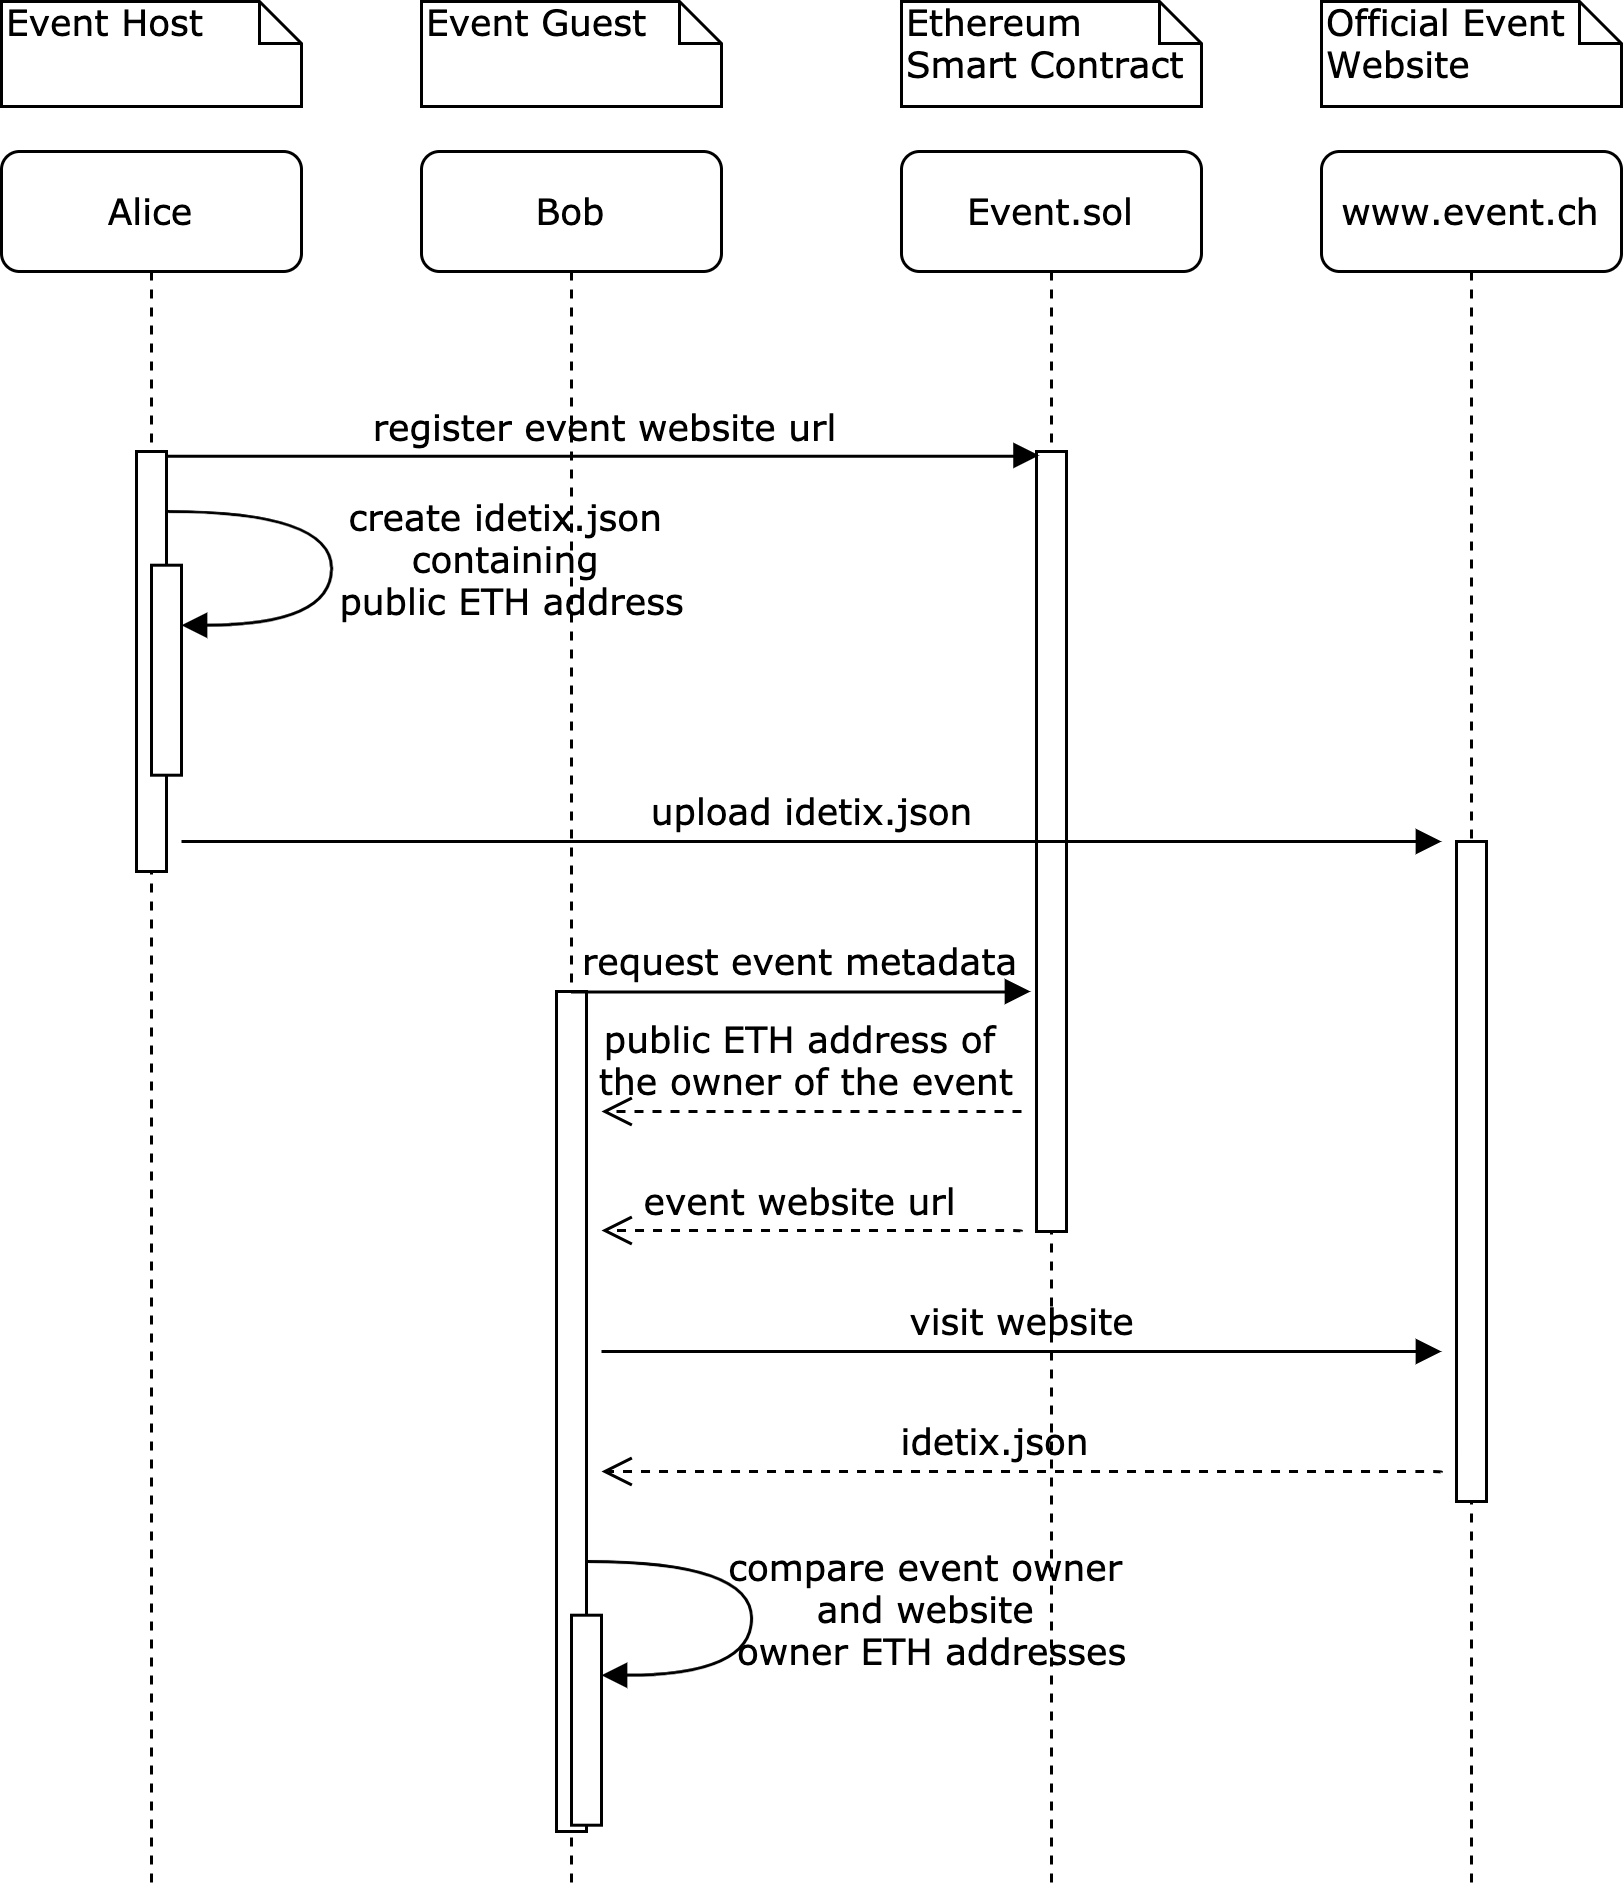
\includegraphics[width=14cm]{figures/social-trust-certificates.png}
    \caption{Social Trust Certificated on the Event Website}
    \label{fig:trust-certificate-event-website}
\end{figure}

Similarly, this procedure can be applied to any social profile such as Twitter, Facebook, Instagram etc. Instead of uploading a JSON file, the public address is included in the profile description on that particular social media platform. 